The following text describes the different classes the Genomizer server uses to communicate with the database and the file system. All the communication with the database happens through the \class{DatabaseAccessor}-class, which uses several helper classes that contain methods with the actual logic. These relationships are visualized in \refer{fig:dat_overview_schema}. 

\begin{figure}[h!]
	\centering
	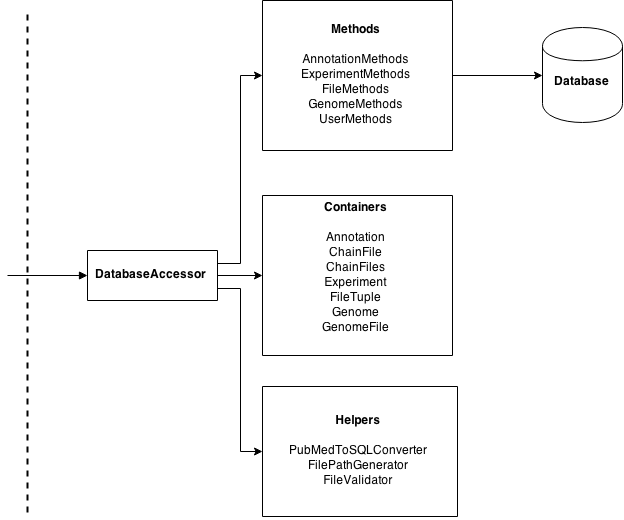
\includegraphics[width=0.67\textwidth]{dat_overview_schema}
%\addImage{dat_overview_schema.png}
\caption{Conceptual overview - The implementation of data access and storage}
\label{fig:dat_overview_schema}
\end{figure}

\subsubsection{DatabaseAccessor}
\class{DatabaseAccessor} is a class that serves as an API for the \term{Genomizer} database - it handles all connections and queries to the database. The methods simplify queries to the database by removing the need to write \term{SQL} in any other packages. For more details see the class diagram, \refer{fig:dat_dbac}, in \refer{chap:dat_umls}.

\subsubsection{Containers}
The classes grouped under the name Containers are used for representation of domain specific objects. An \class{Experiment} is a container for an experiment's annotations and their values as well as a list of files corresponding to that experiment. These files are contained in \class{FileTuple} objects which holds information regarding filename, type, size etc. The \class{Annotation} class contains information about label, whether or not the label is required, the default value and annotation choiches for drop down menus. More information can be found in the class diagram \refer{fig:dat_containers} in \refer{chap:dat_umls}.

\subsubsection{Methods}
The \class{DatabaseAccessor} uses helper classes to execute \term{SQL} queries. These helper classes are grouped by their area of responsibility:
\begin{itemize}
\item Annotation methods
\item Experiment methods
\item File methods
\item Genome methods
\item User methods
\end{itemize}
These classes execute the basic \term{SQL} functions create, read, update and delete (CRUD). The use of \term{prepared statements} (also known as parameterized queries) safeguards against \term{SQL} injection. When modifications to more than one relation are made from a single method, transactions are used to not put the database in an inconsistent state.

\subsubsection{Helpers}
The creation of folders is handled by the \class{FilePathGenerator} class. Folders are created for a new experiment when the experiment is added to the database, including subfolders in preparation of files to be uploaded. All files are divided into folders corresponding to experiment id, except for genome release files that are divided in regards to species.

The \class{PubMedToSQLConverter} class converts a \term{PubMed} string to a \term{SQL} query. The simplest format for a \term{PubMed} string is \term{value[Label]} but the user can enter the annotation labels and values in combination with the the logical operators \texttt{AND}, \texttt{OR} and \texttt{NOT}. Parentheses are used for disambiguation.
\begin{example}
To search for all raw files that Per created the PubMed string should be:

raw[FileType] AND Per[Author]
\end{example}

Searches can be made on labels corresponding to file attributes as well as experiment id. Searching for the empty string will return all experiments in the database.

To validate filename a check against a \term{regex} is done in the \class{FileValidator} class.

\subsubsection{Testing}
WARNING! The unit tests in the \texttt{database.test} package have a database dependency. Do not run any of the tests found in this package on a database that is in use. All tuples are removed from the database upon test completion. Every instance of unit testing should start with an empty database and finish with an empty database to avoid test interdependency.

All the unit tests use the JUnit package and utilize the \class{TestInitializer} class. This simplifies the process of connecting to the test database, filling it with test tuples and clearing the test database and closing the connection when the test class is finished. The individual unit tests can be found in the \texttt{database.test.unittests} package. The scripts for adding the test tuples and clearing the test database tables can also be found in the \texttt{sql} package.